\documentclass{article}
\usepackage{cmap}
\usepackage[utf8]{inputenc}
\usepackage[english,ukrainian]{babel}
\usepackage{graphicx}
\usepackage{geometry}
\usepackage{listings}
\usepackage{float}
\usepackage{amsmath}
\geometry{
	a4paper,
	left=20mm,
	right=20mm,
	top=15mm,
	bottom=15mm,
}
\lstset{
	language=c,
	tabsize=4,
	keepspaces,
	showstringspaces=false,
}
\graphicspath{ {./pictures} }
\setlength{\parindent}{4em}

\newcommand\subject{Архітектура комп'ютера}
\newcommand\lecturer{доцент кафедри ПЗ\\Крук О.Г.}
\newcommand\teacher{доцент кафедри ПЗ\\Крук О.Г.}
\newcommand\mygroup{ПЗ-22}
\newcommand\lab{2}
\newcommand\theme{Синтез та Моделювання шифраторів і дешифраторів та мультиплексорів і демультиплексорів в системіProteus}
\newcommand\purpose{Закріпити практичні навики моделювання логічних схем в середовищі системи програм Proteus; поглибити знання про основні типи комбінаційних схем: шифратори, дешифратори, мультиплексори і демультиплексори; опанувати їх синтез; дослідити роботу синтезованих схем в системі програм Proteus}

\begin{document}
\begin{normalsize}
	\begin{titlepage}
		\thispagestyle{empty}
		\begin{center}
			\textbf{МІНІСТЕРСТВО ОСВІТИ І НАУКИ УКРАЇНИ\\
				НАЦІОНАЛЬНИЙ УНІВЕРСИТЕТ "ЛЬВІВСЬКА ПОЛІТЕХНІКА"}
		\end{center}
		\begin{flushright}
			\textbf{ІКНІ}\\
			Кафедра \textbf{ПЗ}
		\end{flushright}
		\vspace{200pt}
		\begin{center}
			\textbf{ЗВІТ}\\
			\vspace{10pt}
			до лабораторної роботи № \lab\\
			\textbf{на тему}: “\textit{\theme}”\\
			\textbf{з дисципліни}: “\subject”
		\end{center}
		\vspace{112pt}
		\begin{flushright}
			
			\textbf{Лектор}:\\
			\lecturer\\
			\vspace{28pt}
			\textbf{Виконав}:\\
			
			студент групи \mygroup\\
			Коваленко Д.М.\\
			\vspace{28pt}
			\textbf{Прийняв}:\\
			
			\teacher\\
			
			\vspace{28pt}
			«\rule{1cm}{0.15mm}» \rule{1.5cm}{0.15mm} 2022 р.\\
			$\sum$ = \rule{1cm}{0.15mm}……………\\
			
		\end{flushright}
		\vspace{\fill}
		\begin{center}
			\textbf{Львів — 2022}
		\end{center}
	\end{titlepage}
		
	\begin{description}
		\item[Тема.] \theme.
		\item[Мета.] \purpose.
	\end{description}

	\section*{Індивідуальне завдання}
\begin{figure}[H]
		\centering
		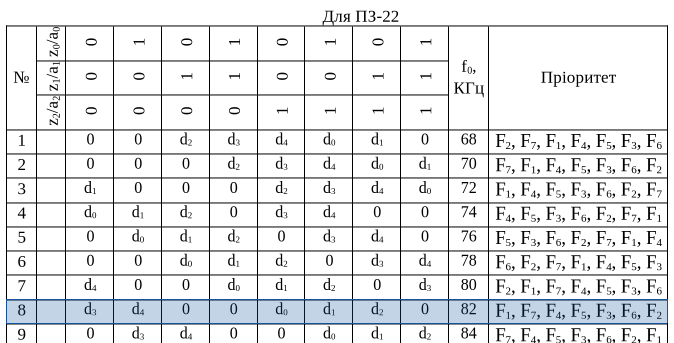
\includegraphics[scale=0.75]{v}
	\end{figure}	

	\section*{Теоретичні відомості}
	
	
	\section*{Хід роботи}
	\begingroup
	\setlength{\belowdisplayskip}{-15pt}
	\setlength{\abovedisplayskip}{0pt}
	\subsection*{Період цифрового сигналу}
	\begin{large}
		\begin{gather}
			T=\frac{1}{f};\hspace{22mm}T=\frac{1}{82\text{кГц}}=\frac{1}{82000\text{Гц}}=0.0000121\text{с}\nonumber\\
			\tau=\frac{T}{8}=0.00000151\text{с}\nonumber
		\end{gather}
	\end{large}
	\subsection*{ДДНФ заданої функції}
	\begin{large}
		\begin{gather}
			F=\overline{x_2}\overline{x_1}\overline{x_0}+\overline{x_2}\overline{x_1}x_0+x_2\overline{x_1}\overline{x_0}+x_2\overline{x_1}x_0+x_2x_1\overline{x_0}	\nonumber
		\end{gather}
	\end{large}
	\endgroup
	
	\begin{figure}[H]
		\centering
		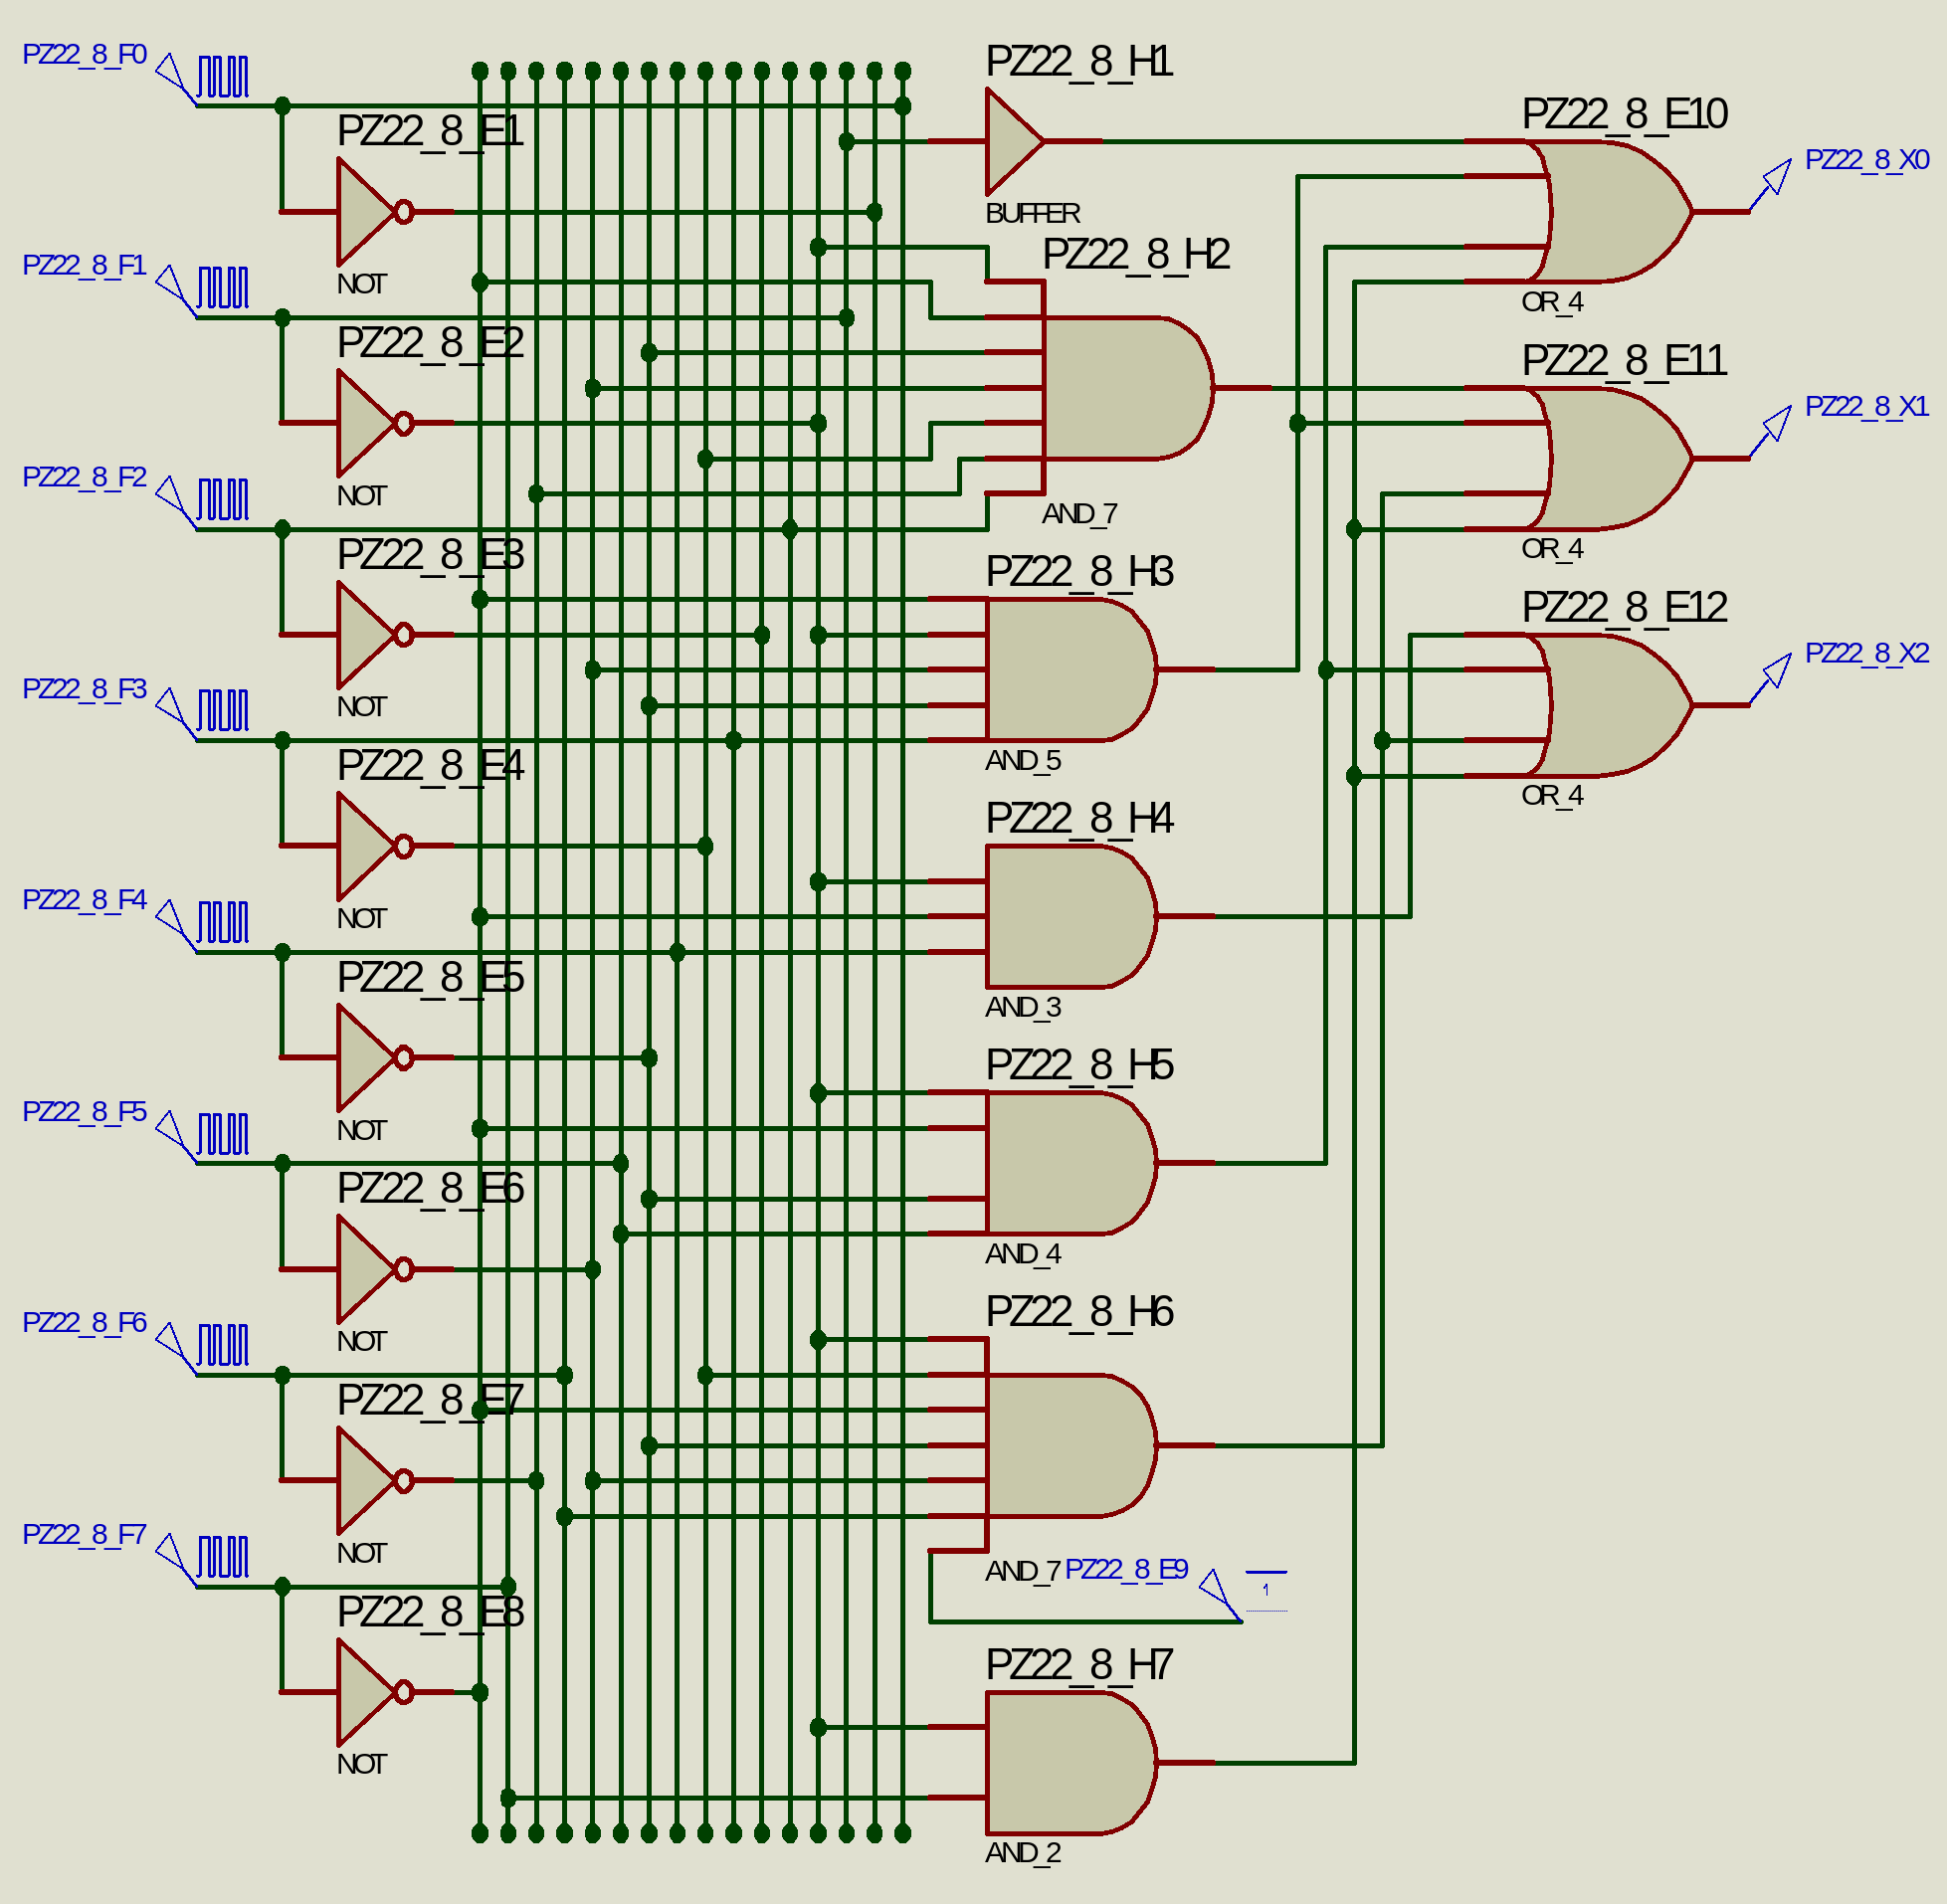
\includegraphics[scale=0.25]{s1}	
		\caption{Схема 1}
	\end{figure}
	\begin{figure}[H]
		\centering
		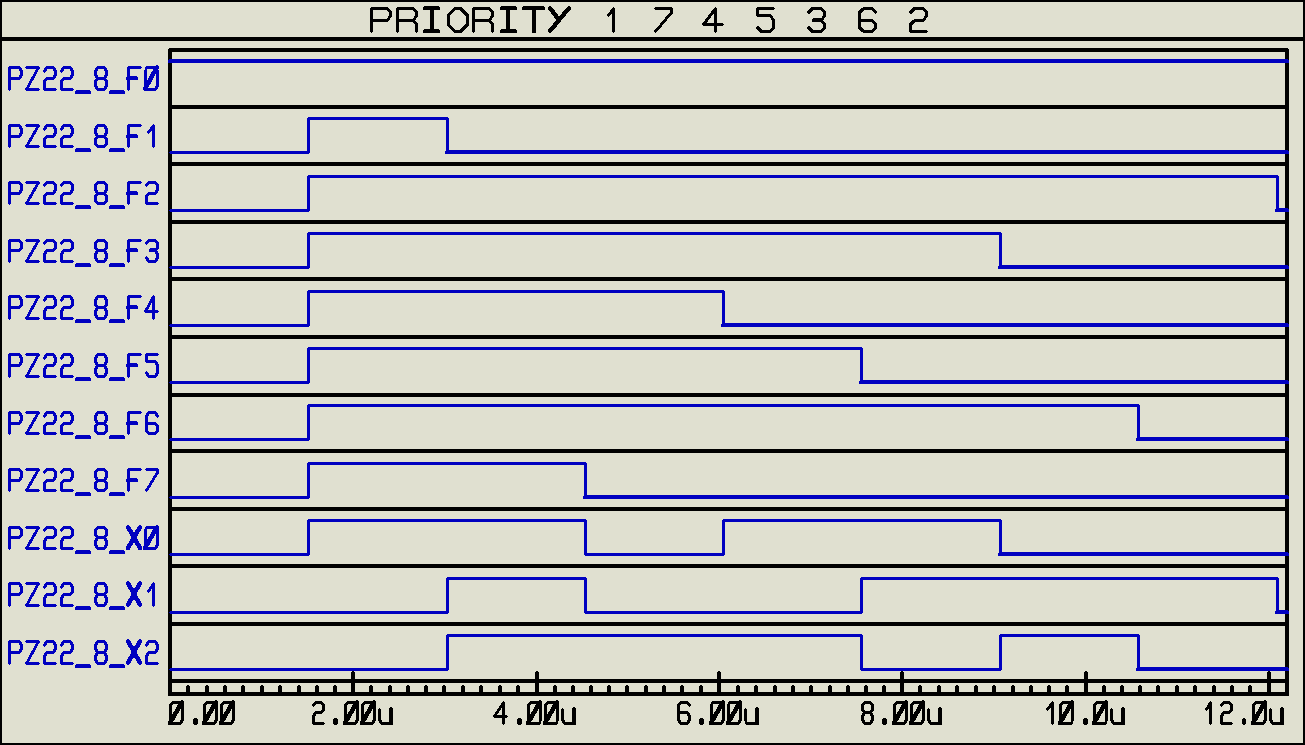
\includegraphics[scale=0.34]{g1}	
		\caption{Графік 1}
	\end{figure}

	За отриманим графіком виконання схеми пріоритетного шифратора видно, що заданий пріоритет є таким: 1, 7, 4, 5, 3, 6, 2, що повністю співпадає з заданим варіантом, отже, можна зробити виновок, що моделювання виконано правильно.

	\begin{figure}[H]
		\centering
		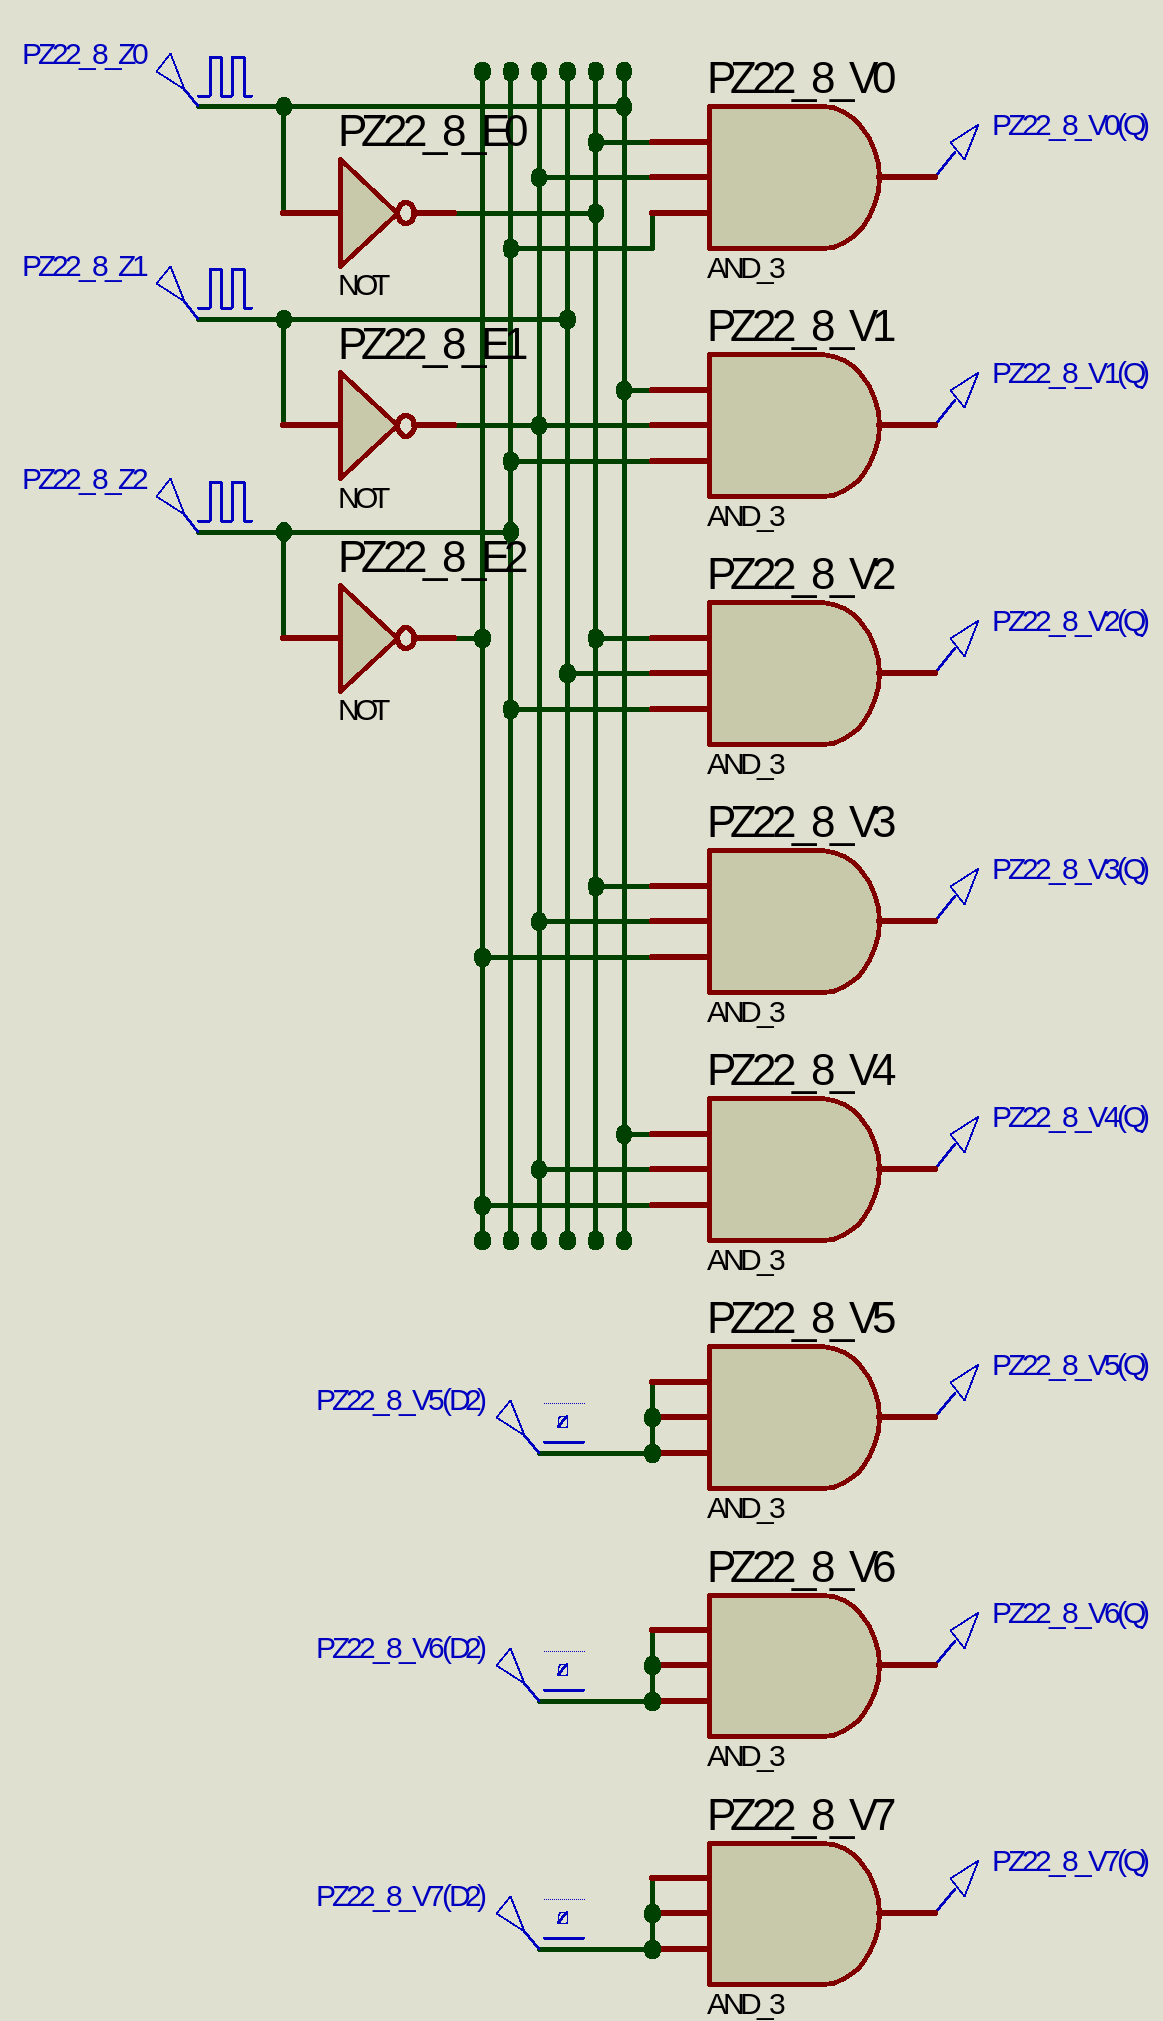
\includegraphics[scale=0.34]{s2}	
		\caption{Схема 2}
	\end{figure}
	\begin{figure}[H]
		\centering
		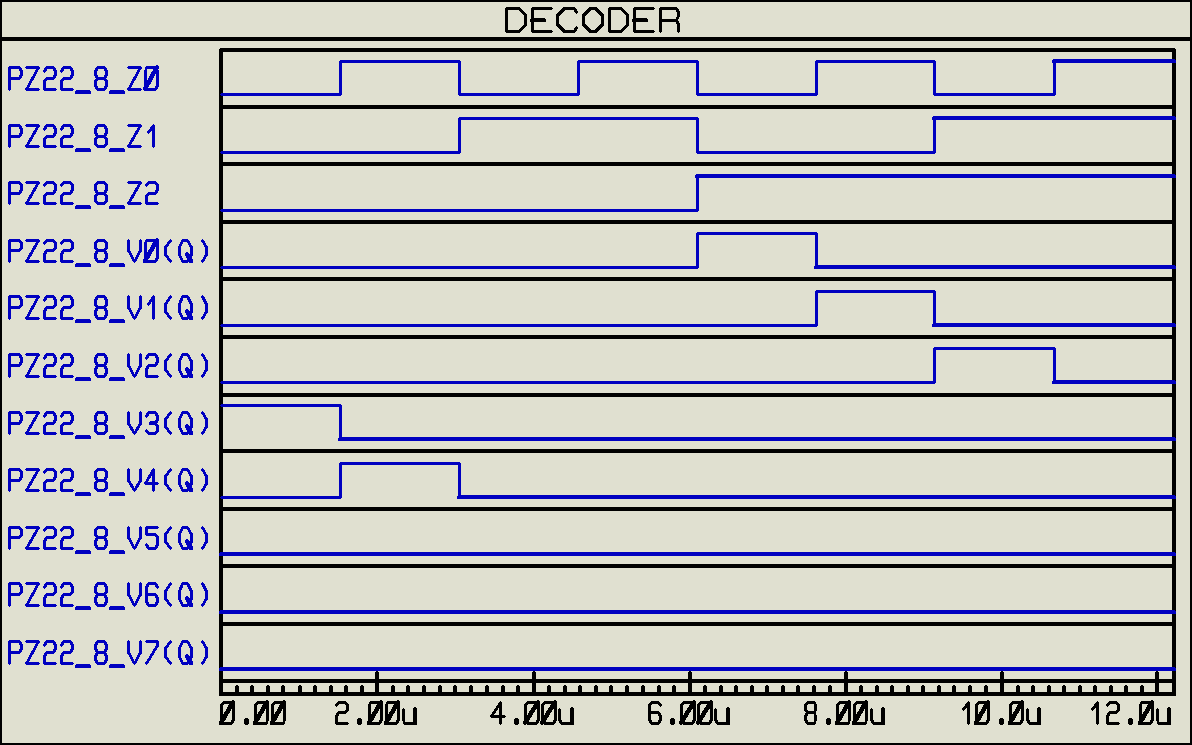
\includegraphics[scale=0.34]{g2}	
		\caption{Графік 2}
	\end{figure}

	\begin{figure}[H]
		\centering
		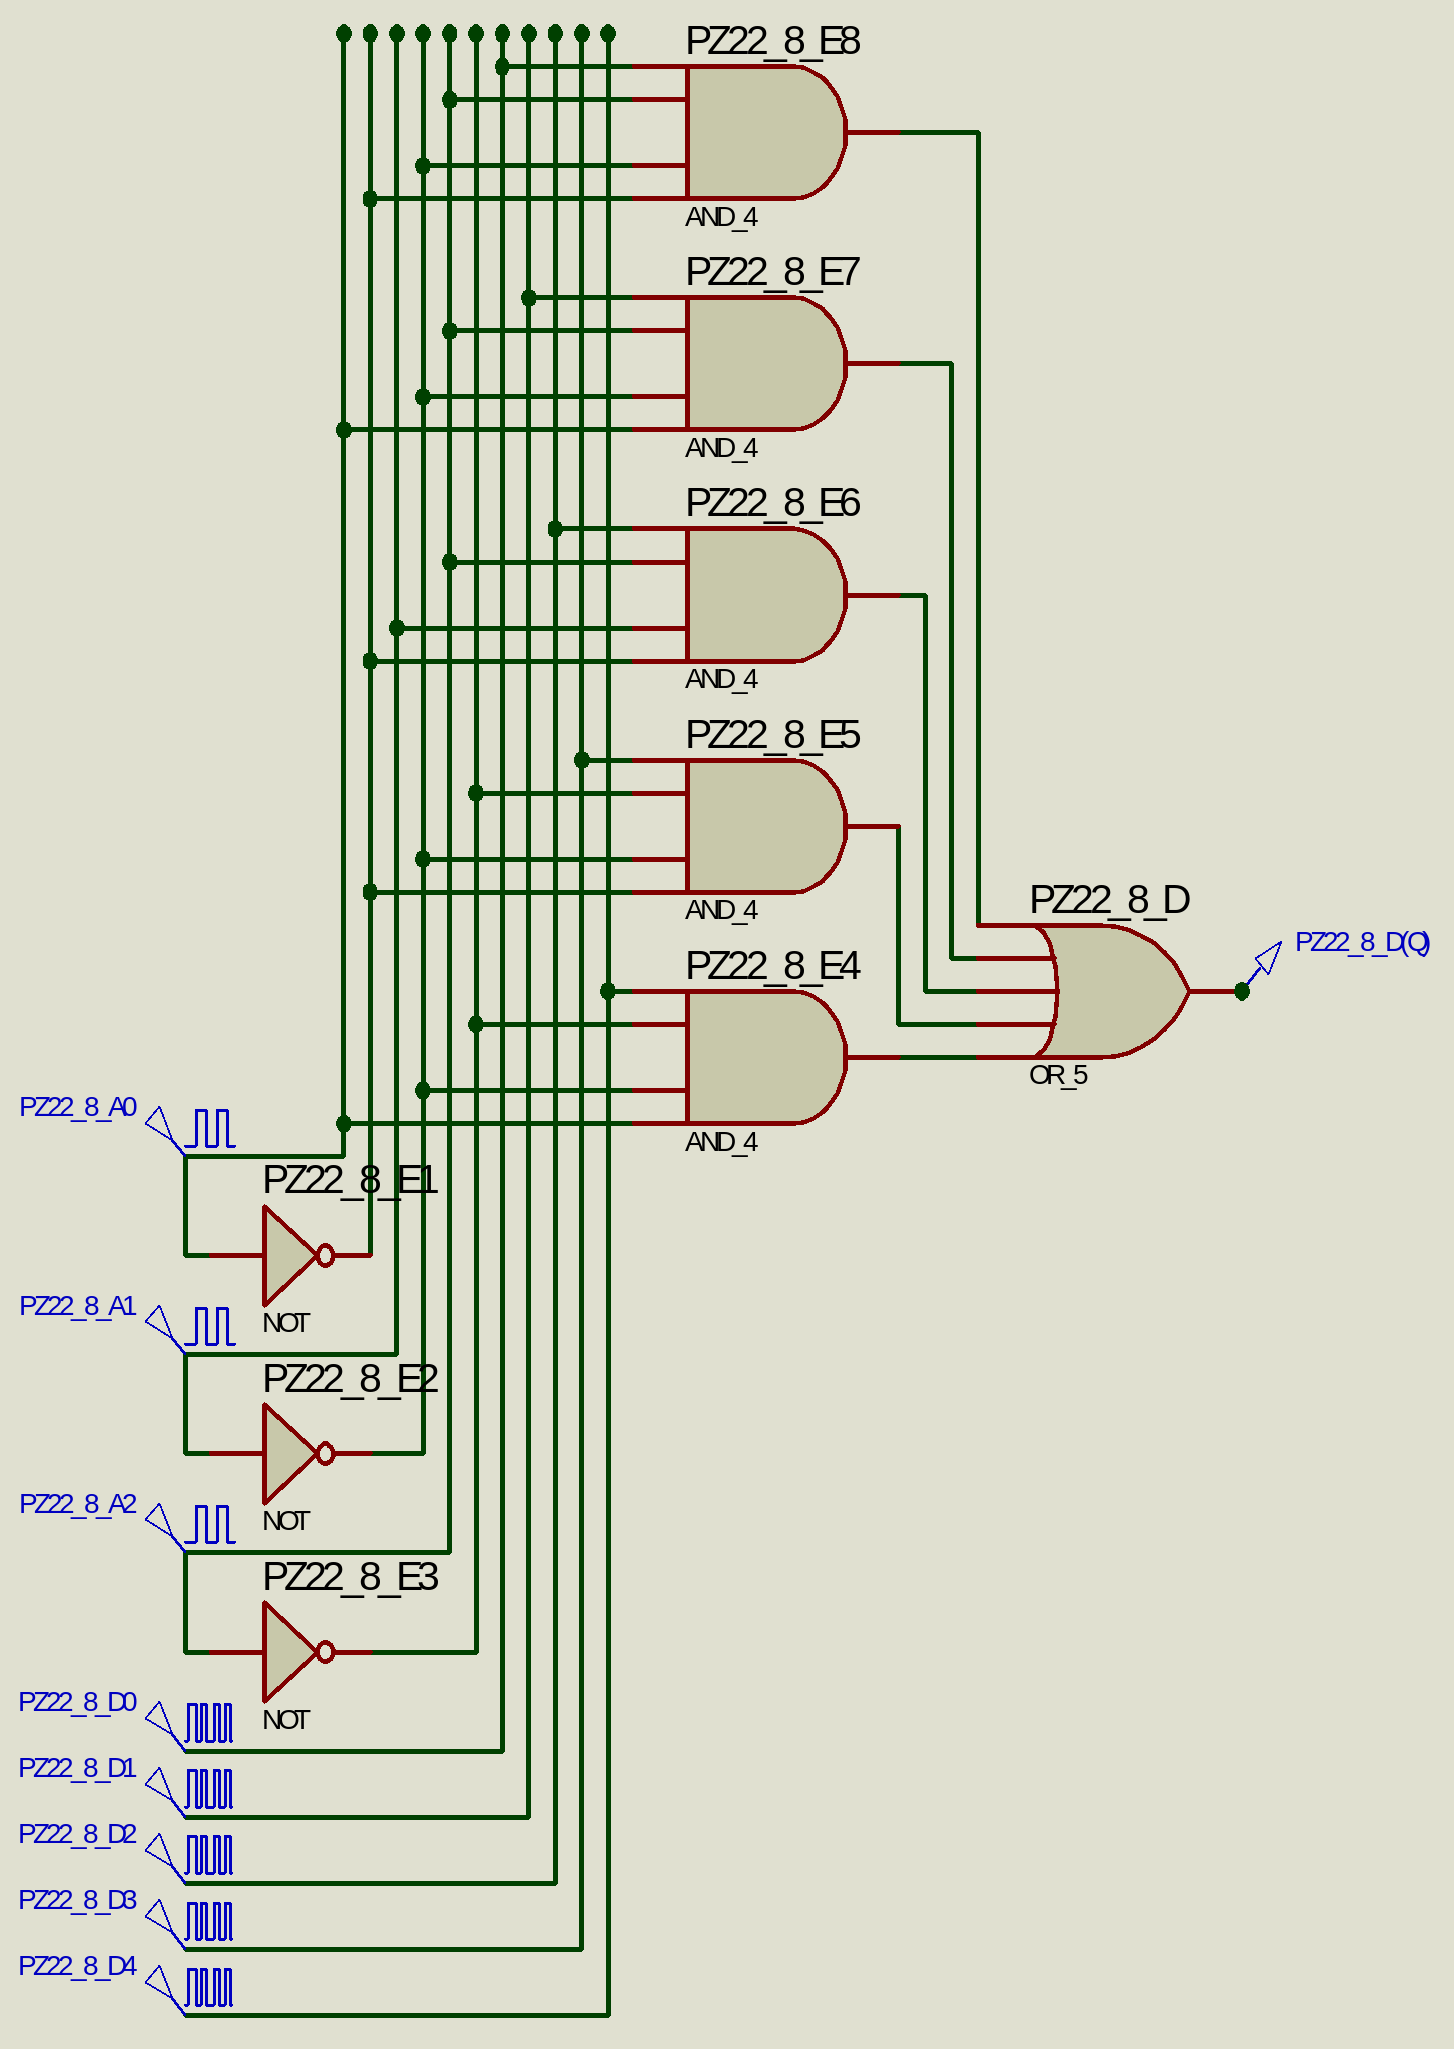
\includegraphics[scale=0.34]{s3}	
		\caption{Схема 3}
	\end{figure}
	\begin{figure}[H]
		\centering
		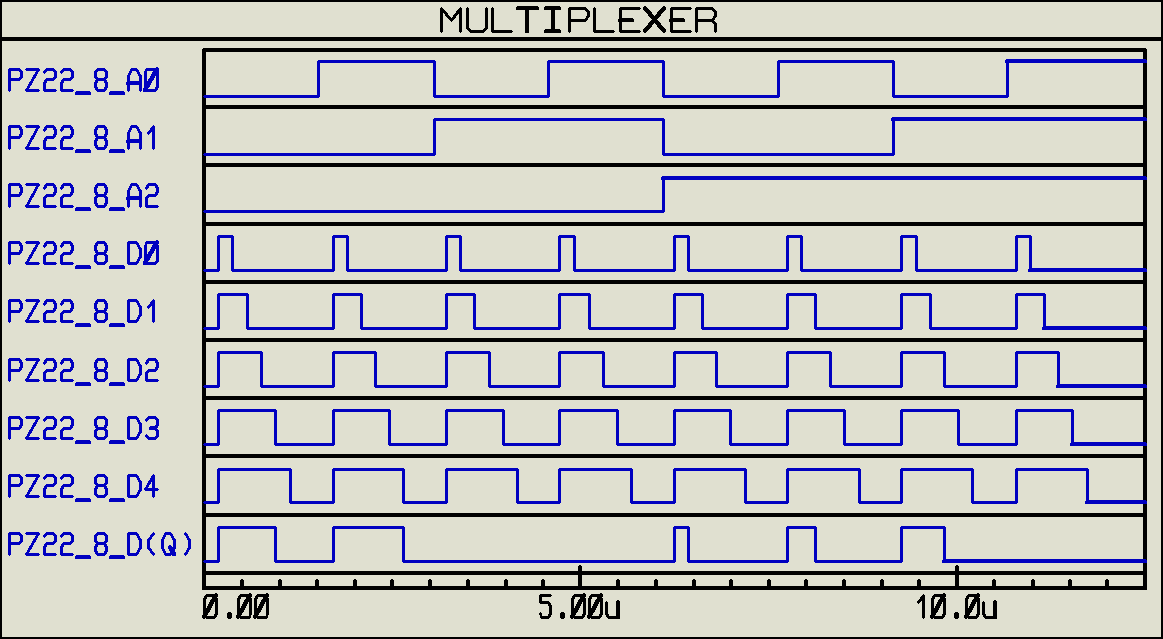
\includegraphics[scale=0.34]{g3}	
		\caption{Графік 3}
	\end{figure}

	\begin{figure}[H]
		\centering
		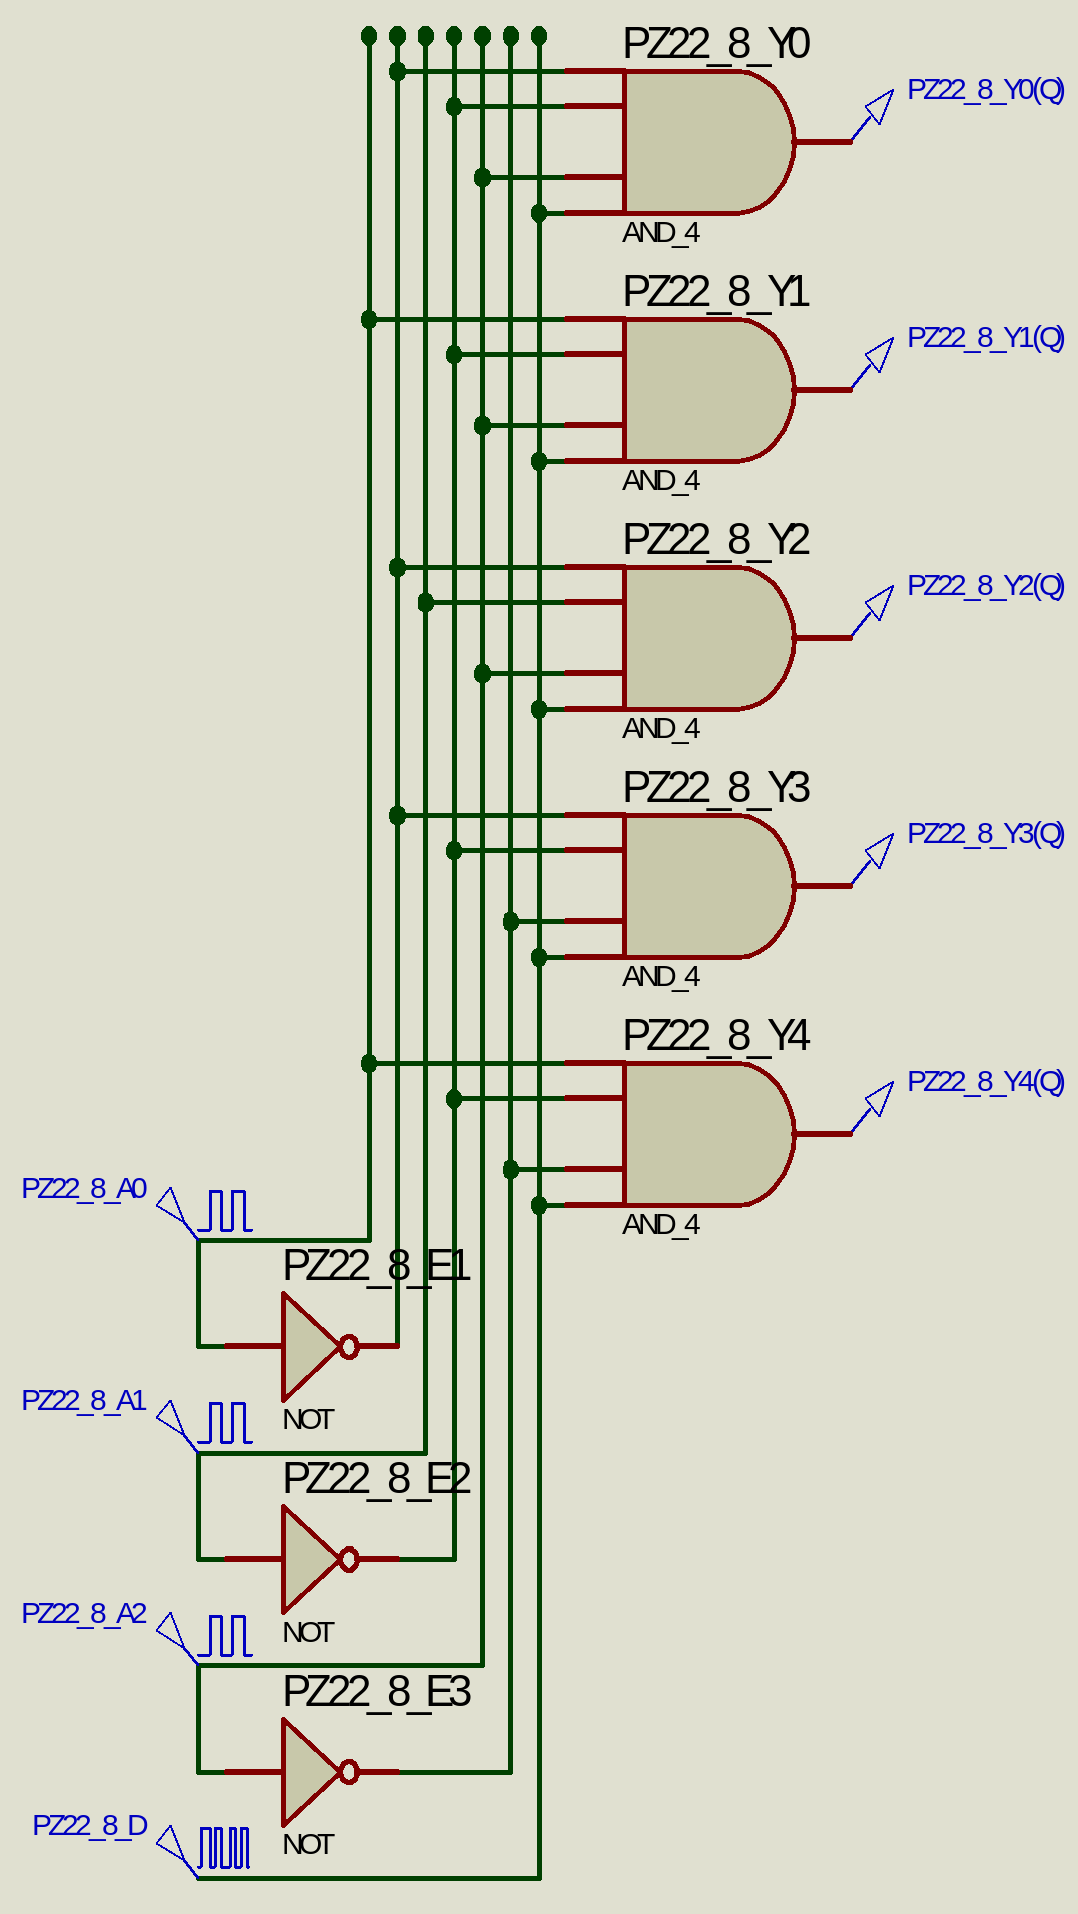
\includegraphics[scale=0.34]{s4}	
		\caption{Схема 4}
	\end{figure}
	\begin{figure}[H]
		\centering
		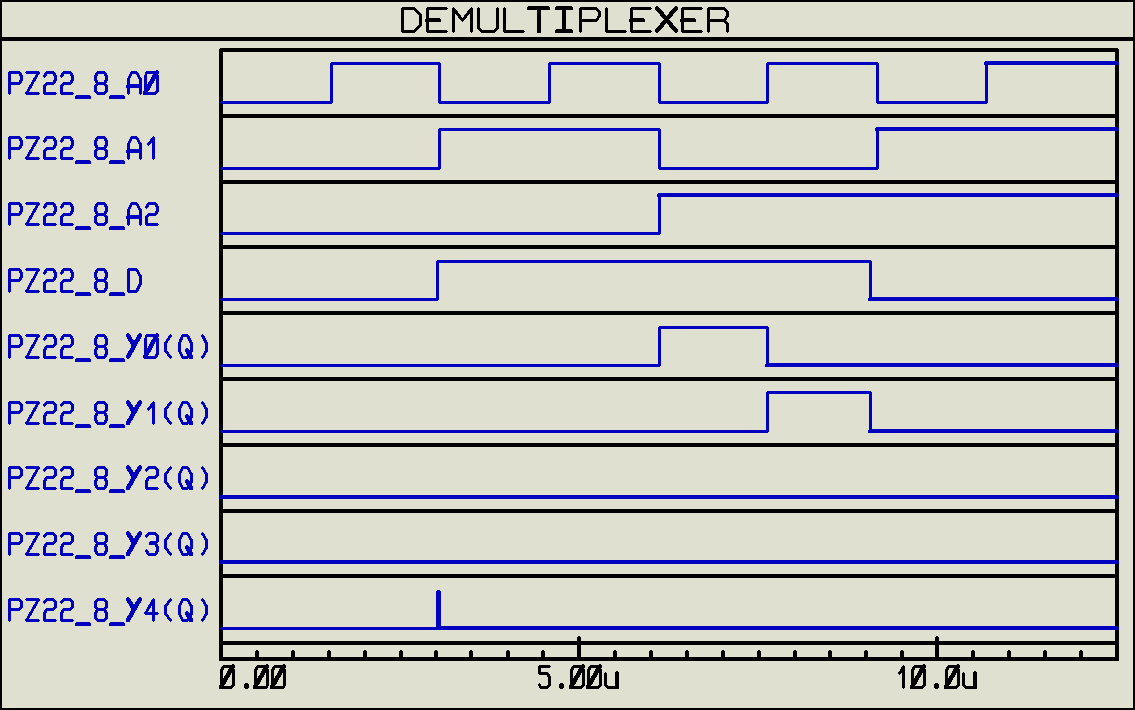
\includegraphics[scale=0.34]{g4}	
		\caption{Графік 4}
	\end{figure}

	\section*{Висновки}
	Під час виконання лабораторної роботи я закріпив практичні навики моделювання логічних схем в середовищі системи програм Proteus. 
	Поглибив знання про основні типи комбінаційних схем: шифратор, дешифратор, мультиплексор і демультиплексор. Опанував їх синтез. 
	
	Дослідив роботу синтезованих схем в системі програм Proteus. Змоделював графіки цих схем за заданим варіантом.
	    
\end{normalsize}
\end{document}
